
\documentclass[12pt]{report}

\usepackage{bitsetup}

%=============== START OF THE DOCUMENT
\begin{document}
\onehalfspacing

%=============== SETUP: PARAGRAPH STYLES
\setlength{\parindent}{3em} % start indentation
\setlength{\parskip}{1em} % vertical space between two paragraphs

%========= PAGE: TITLE PAGE (COVER)
\thispagestyle{empty}
\begin{titlepage}
	\begin{center}
		\vspace*{2cm}
		\includegraphics[width=0.15\textwidth]{uoc/uocLogo.jpg}\\
		\vspace{1cm}
		{\LARGE Sales and Production Management System for \\Two Elephants Fireworks}
		\vspace{2cm}
		\begin{large}

			\textbf{D.A.N.P. DISSANAYAKE}\\
			\vspace{2cm}
			BIT Registration Number: R181344 \\
			Index Number: 1813447 \\
			Name of the Client :  Onelli Traders / Two Elephants Fireworks \\
			Name of the supervisor :  J.A. Manjula Sanjeewa \\

			\vspace{1cm}

			\bf{2020/ August}

			\vspace{2.5cm}

			\vfill


			\includegraphics[width=0.15\textwidth]{uoc/ucscLogo.png}%
			\begin{minipage}[b]{0.7\textwidth}
				\centering
				{\small \bf Degree of \acrlong{bit} of the \acrlong{ucsc}}
			\end{minipage}%
			\includegraphics[width=0.15\textwidth]{uoc/bitLogo.png}
		\end{large}
	\end{center}
\end{titlepage}

%========= PAGE: DECLARATION
\newpage
\thispagestyle{plain}
\pagenumbering{roman}
\setcounter{page}{2}
\chapter*{\Huge Declaration}
\addcontentsline{toc}{chapter}{\bf{Declaration}}

\noindent
\fbox{\includegraphics[width=\textwidth]{declaration.png}}

%========= PAGE: ABSTRACT
\newpage
\thispagestyle{plain}
\chapter*{\Huge Abstract}
\addcontentsline{toc}{chapter}{\bf{Abstract}}

Two Elephants Fireworks is a gun-powder based product manufacturing company in Walpala. Their products range from firecrackers to high-power fireworks for large scale events. Currently, employees in this company have to deal with manually maintaining multiple lists of transactions, products, and material details. There is no way to store and keep track of customer details at the moment and generating reports to make business decisions, observe growth and customer demands is really hard due to the nature of these manual processes.

Since the current system is manual, it is very difficult to manage daily sales, orders, material details, the billing process, and the rest of their daily operations. Having to maintain and keep track of hundreds of books and papers makes it very hard and time-consuming to fulfill customer orders and causes some customers to wait for a long period of time. Since manually keeping track of the inventory is needed, it consumes a lot of manpower and time. Furthermore, due to human errors, there is a considerable amount of late order deliveries. The owner of this company is also having trouble checking recent orders and sales information while he is traveling.

Taking the above issues into consideration, the proposed system is being developed for a web-based environment. It aims to make it easy to manage their business processes while introducing better mechanisms to improve their efficiency. This system supports users, privileges, and report generating for making business decisions. Not only that but also this will facilitate remote access to the system making it possible to check recent information without having to come to the office.

Visual Studio Code is being used to develop the proposed system in TypeScript and JavaScript languages. MySQL and TypeORM are used to manage the data storing and retrieving aspect of the system along with Chart.js and Datatables to facilitate the report generating process. Furthermore, \acrlong{uml} was used for the analysis and design processes and this system is being developed according to the \acrshort{mvc} architecture using iterative and incremental approach.

This proposed system will achieve the client's functional and non-functional requirements by providing an efficient and user-friendly environment. Also, this will provide tools to optimize business processes and make decisions based on more accurate reports and data.

%========= PAGE: Acknowledgment
\newpage
\thispagestyle{plain}
\chapter*{\Huge Acknowledgment}
\addcontentsline{toc}{chapter}{\bf{Acknowledgment}}
I would like to take this space to acknowledge and extend my heartiest gratitude to those who have helped me in various ways throughout this project to make it a success.

First and foremost, I owe my deep gratitude to the University of Colombo School of Computing for offering us this precious degree program and qualified individuals to guide us until graduation.

Very special recognition should be given to my project supervisor Mr. J.A. Manjula Sanjeewa and Mr. Haritha Pramodha for their extensive assistance, guidance, and valuable support throughout the project period. Without their support, the completion of this project would have been extremely complicated. I also take this opportunity to thank Mr. N.R. Fernando, the manager of Two Elephant Fireworks and the rest of the staff, gave me the opportunity to develop this system.

It is my duty to thank Mr. Haritha Pramodha, Mr. Manjula Jayasinghe, Mr. Susith Sanasuma, and the rest of the lecture panel of W3 Campus for helping me to gain academic knowledge for the BIT degree program and allowing me to use the college resources throughout this period. Also, I thank all of my friends and colleagues who have helped me in numerous ways and encouraged me to complete the project successfully.

Finally, I thank my family members for their unconditional love and support given in every way possible throughout the years of this degree program.


%========== PAGE: TABLE OF CONTENT
\newpage
\addcontentsline{toc}{chapter}{\bf{Contents}}
\begin{singlespacing}
	\tableofcontents
\end{singlespacing}
\setlength{\parskip}{1em}
\renewcommand{\baselinestretch}{2.0}


%========== PAGE: LIST OF FIGURES
\newpage
\addcontentsline{toc}{chapter}{\bf{List of Figures}}
\begin{singlespacing}
	\listoffigures
\end{singlespacing}
% \setlength{\parskip}{1em}
\renewcommand{\baselinestretch}{2.0}


%========== PAGE: LIST OF TABLES
\newpage
\addcontentsline{toc}{chapter}{\bf{List of Tables}}
\begin{singlespacing}
	\listoftables
\end{singlespacing}
% \setlength{\parskip}{1em}
\renewcommand{\baselinestretch}{2.0}


%========== PAGE: LIST OF ACRONYMS
% \section*{\Huge List of Acronyms}
% \addcontentsline{toc}{chapter}{\bf{List of Acronyms}}
\newpage
\addcontentsline{toc}{chapter}{\bf{List of Acronyms}}
\begin{doublespace}
	\printglossary[type=\acronymtype,title={\Huge List of Acronyms}]
\end{doublespace}

% \setlength{\parskip}{1em}
% \renewcommand{\baselinestretch}{2.0}


%================ SETUP: SECTION TITLE FONT SIZES
\titleformat*{\section}{\fontsize{16}{19}\bfseries\normalfont}
\titleformat*{\subsection}{\fontsize{14}{17}\bfseries\normalfont}
\titleformat*{\subsubsection}{\fontsize{12}{15}\bfseries\normalfont}

%>>>>>>>>>>>>>>>>>>>>>>>>>>>>>>>>>>>>>>>>>>>>>>>>>>>>>>>>
% Main body of Thesis
%========= Start of Thesis 
\newpage
\pagenumbering{arabic}
\setcounter{page}{1}
\setcounter{secnumdepth}{3} % enable subsubsection numbering
\onehalfspacing

\chapter{Introduction}
This chapter introduces background information of the selected company for the project, the problems going to be solved, objectives hoping to accomplish, and the scope of the project.

\section{Motivation}
Two Elephants Fireworks is one of the major gun-powder based product manufacturers in the Andiambalama. But currently, all of their processes and paperwork are done manually. Due to the high number of clients and suppliers, managing all of their operations this way has become a very time-consuming inefficient task. Below are some of the difficulties they have to face because of their current way of performing tasks.

\begin{itemize}
	\item There is no proper way to manage customer details, so they have to request same details over and over again.
	\item Customer order management process is very time-consuming and inconsistent.
	\item They are unable to properly calculate measurements of raw materials needed to complete an order.
	\item Lot of materials and processed materials go to waste because there is no way to properly keep track of the inventory.
	\item There is no way to generate reports about sales and inventory to make business decisions such as when to increase the production \& supply.
	\item There is no procedure to manage payments, installments and payment history.
	\item it is difficult to find required information quickly because there are lots of files and paperwork to go through.
\end{itemize}

In order to provide a reliable solution that can address the above issues, I wish to develop a computer-based sales and production management system. This system will be able to improve the profits, efficiency of daily operations, and overall customer satisfaction by reducing complexities and providing better solutions to existing business processes.

\section{Aims \& Objectives of the Project}

The intent of this computer-based system is to provide a reliable solution for existing drawbacks.  This system hopes to achieve the following objectives in order to improve the state of current operations.

\begin{itemize}
	\item Reduce material and inventory waste by switching to a database approach.

	\item Improve the efficiency of inventory management process.

	\item Provide a way to easily calculate raw material for production with the help of inventory.

	\item Provide the ability to manage and access customer details efficiently.

	\item Provide a reliable,  trustworthy and consistent way to manage payment details.

	\item Provide a mechanism to easily generate reports for making decisions.

	\item Reduce costs by eliminating the need to store information physically.

	\item Generate receipts accurately and easily for tasks such as making a new sale.

	\item Reduce employee workload by providing features to simplify complex processes.

	\item Help this business to gain competitive advantage by allowing access to more accurate information.
\end{itemize}

\section{Scope of the Project}
The scope of this system covers the sales and production area of this business according to their requirements. Below are the details that will be managed by the proposed system.

\begin{itemize}
	\item {\bf{Manage customer details.}}\\
	      This will facilitate storing and managing customer details including their names, credit limits and contact details.

	\item {\bf{Manage item details.}}\\
	      All individual items and information related to each item will be stored and manageable.

	\item {\bf{Manage product details.}}\\
	      Since items are not sold individually, this will facilitate storing and managing details about item packs.

	\item {\bf{Manage purchase order details.}}\\
	      Ordering new materials needed for production from suppliers and managing those orders will be possible. These purchase orders
	      will also be stored.

	\item {\bf{Manage raw material details.}}\\
	      Information regarding raw materials needed to produce items will be stored and manageable.

	\item {\bf{Manage supplier details.}}\\
	      This will facilitate storing and managing supplier information and their contact details.

	\item {\bf{Manage payment details.}}\\
	      Payments done by customers and payments done to suppliers will be stored. History of these payments will also be accessible.
	\item {\bf{Generate reports.}}\\
	      This module will allow user to generate reports related to various areas such as sales, inventory and supplies easily.

	\item {\bf{Generate bills.}}\\
	      This module will generate detailed bills for customers who purchase products.

	\item {\bf{Manage employee details.}}\\
	      This will facilitate storing and managing employee details such as their names, contact details and status.

	\item {\bf{Manage roles.}}\\
	      This module will facilitate creating, modifying and deleting of roles for users of the system.

	\item {\bf{Manage role privileges.}}\\
	      Privileges each role have over each module of the system is customized through this facility. This can be used to restrict or allow access to individual parts of the system.
\end{itemize}

\newpage
\chapter{Analysis}

Requirement analysis is the first and most critical stage in the \acrlong{sdlc}. The success of all other stages heavily depends on the information gathered in this phase. Requirement analysis is the process of identifying users and their duties, understanding the problem domain, and understanding user requirements.

The requirements should be documented, measurable, testable, traceable, related to identified business needs or functionalities, and defined to a level of detail sufficient for system design \cite{sommerville_2008_se}.

After collecting requirements through various methods they are classified into two categories called functional requirements and non-functional requirements. Furthermore, how much of the actual idea can be implemented will also be considered in this phase.

\section{Review of similar systems with references}
By observing existing web-based solutions to similar domains more experience can be obtained on how our proposed system should be developed and how required features should be presented to the user.  Following are a few of the systems that were reviewed before starting building this system.

\subsection{Sales and Inventory Management System in Dineth Stores}
This store owner uses their web-based system in order to manage their sales and inventory. This system consists of multiple views allowing users of the system to easily interact and perform tasks.  Furthermore, this system has an online shop feature customers can use to directly place their orders.

The following figure shows the dashboard of their web-based system. This is the welcome screen users see when they logged into the system. This can also be considered as the home page. It contains various useful information such as the number of items in the inventory, total orders, and total products. Also, users can quickly get more detailed information just by clicking on one of these cards.

\begin{figure}[H]
	\centering
	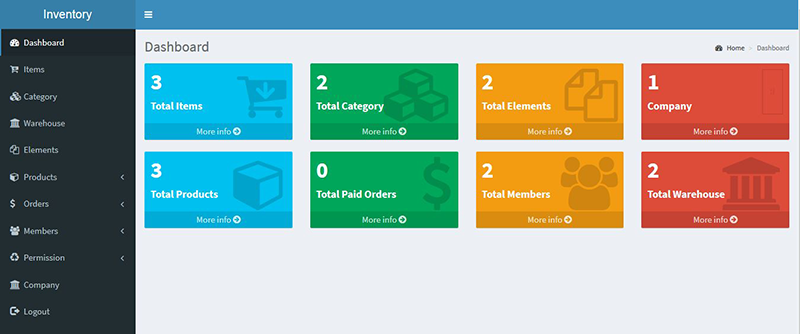
\includegraphics[width=1\textwidth]{simillarSystems/dineth1.png}
	\caption{Dashboard of the Sales and Inventory Management System in Dineth Stores}
\end{figure}

\subsection{Sales management system in Shaanthi Grocery}

This grocery store owner uses their sales management system to perform daily transactions and keep track of history regarding sales.  Furthermore, it has facilities to keep track of the inventory, manage purchase orders and manage purchase returns.

\begin{figure}[H]
	\centering
	\includegraphics[width=1\textwidth]{simillarSystems/shaanthi1.png}
	\caption{Item Management Window of the Sales Management System in Shaanthi Grocery}
\end{figure}

\begin{figure}[H]
	\centering
	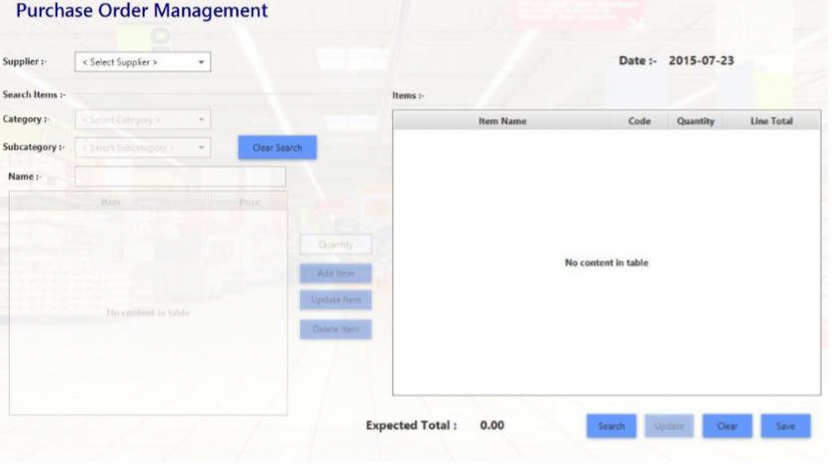
\includegraphics[width=1\textwidth]{simillarSystems/shaanthi2.png}
	\caption{Purchase Order Window of the Sales Management System in Shaanthi Grocery}
\end{figure}

\subsection{Comparison between similar systems}
\begin{table}[H]
	\centering
	\begin{tabular}{ |p{4.5cm}|p{3cm}|p{3cm}|p{2cm}| }
		\hline
		\bf{Features}             & \bf{CBIS in Dineth Stores} & \bf{CBIS in Shaanthi Grocery} & \bf{Proposed System} \\
		\hline
		Item and Supplier Details & Yes                        & Yes                           & Yes                  \\
		\hline
		Employee Details          & Yes                        & No                            & Yes                  \\
		\hline
		Purchase Orders           & Yes                        & Yes                           & Yes                  \\
		\hline
		Manage Sales              & Yes                        & Yes                           & Yes                  \\
		\hline
		Payments and Receipts     & Yes                        & Yes                           & Yes                  \\
		\hline
		\acrshort{grn} Management & Yes                        & Yes                           & Yes                  \\
		\hline
		Generate reports          & Yes                        & Yes                           & Yes                  \\
		\hline
		Notifications reports     & Yes                        & No                            & Yes                  \\
		\hline
	\end{tabular}
	\caption{Comparison between similar systems}
\end{table}

\section{Explaining the current system using diagrams}
The current system with file-based approach stores all records in physical papers. Due to this procedure, it takes a long time to process transactions. Since this organization deals with a huge amount of data, manipulation and retrieval of existing records have become very inefficient.

Furthermore, when new sales are made or customer payment accepted, inventory and payment details need to be manually updated in multiple places. When issuing purchase orders, accepting \acrshort{grn}s and ordering supplies there is a great deal of paperwork that needs to be done. Also, management has difficulties finding necessary reports and data due to the large amount of unorganized paperwork. The following figure briefly shows the existing manual system.

\begin{figure}[H]
	\centering
	\includegraphics[width=\textwidth]{uml/usecaseManual.jpg}
	\caption{Use Case Diagram of the current manual system}
\end{figure}

\section{Identifying the functional and non-functional requirements}

\subsection{Requirement gathering techniques}
In order to capture functional and non-function requirements of the existing system, following techniques were used.

\begin{itemize}
	\item Observation
	\item Document Analysis
	\item Interviews
\end{itemize}

\subsection{Functional Requirements}
Functional requirements specify features developers must implement in order to allow users to accomplish their tasks (user requirements).  These should describe the business requirements end-users are expecting. Following is the list of functional requirements found in this system.

\begin{itemize}
	\item {\bf{Manage item details}} \\
	      It must be possible to store large amount of items with their information and easily search, edit and delete if the need arises.

	\item {\bf{Manage customer details}} \\
	      Since this business deals with hundreds of customers, system must facilitate features to store and manage customer information making it easy and fast for customers to make their purchases.

	\item {\bf{Manage employee details}} \\
	      It should be possible to store and manage past and present employee details with their personal information. Also, handling details such as their current employee status must be possible as well.

	\item {\bf{Manage purchase order details}} \\
	      Making purchase orders through the system must also be possible. Furthermore, system must facilitate managing purchase orders and viewing past orders if needed.

	\item {\bf{Manage \acrshort{grn}s}} \\
	      System must provide an easy-to-use way to manage and store \acrlong{grn}s.

	\item {\bf{Manage material details}} \\
	      Since various materials are used for the production process, it must be possible to store and manage material information in the system. Also, required materials for each individual item should be easily accessible as well.

	\item {\bf{Manage product details}} \\
	      System must provide features to store and manage information about products because items are sold to customers as products or item packages.

	\item {\bf{Manage users}} \\
	      System must facilitate creating and managing users. It must also provide features to set roles for each individual user.

	\item {\bf{Manage roles}} \\
	      Since users have different access levels, system should provide features to create new roles and manage existing ones.

	\item {\bf{Manage role privileges}} \\
	      System must provide a way to grant or restrict privileges for each role easily.

	\item {\bf{Generate reports}} \\
	      Since reports are important for making business decisions and observing growth, system must provide a way to generate custom reports for things such as sales and costs.

	\item {\bf{Generate bills}} \\
	      A bill with details such as item name, quantity and price should be issued through the system for important transactions.

\end{itemize}

\subsection{Non-Functional Requirements}
Non-functional requirements describe the features this system should have. Non-functional requirements are difficult to work with than functional ones because they depend on each user's perspective and preferences. But, the user-friendliness of the system depends on how well these non-functional requirements are met. Following is the list of non-functional requirements aim to offer in the proposed system.

\begin{itemize}
	\item {\bf{Security}}\\
	      Since system will store sensitive details such as personal employee details, there are security measures in place such as user access management, privileges control and unauthorized accedes prevention.

	\item {\bf{Usability}}\\
	      System user-interface contain easy to navigate menus, dashboard and a clear way to indicate the current location user is in. This maximizes the usability of the system allowing user to switch between modules seamlessly.

	\item {\bf{Accuracy}}\\
	      Proposed system has mechanisms in place to handle transactions with minimum error probability allowing users to perform their tasks and retrieve information with high accuracy.

	\item {\bf{User-friendliness}}\\
	      User-interface of the system is very simple and easy to navigate allowing even a new user to learn to perform tasks very quickly.

	\item {\bf{Efficiency and consistency}}\\
	      System has very fast response rates and accurate database management mechanisms preventing issues such as data inconsistencies and slow data retrieval.
\end{itemize}

\section{Justification for the choice of the development life cycle}
Due to the nature of the requirements of this system, an iterative and incremental approach was selected as the development methodology. The most prominent reason for this was the unclear nature of requirements and the complexity of operations in the existing manual system.

Furthermore, actors involved in this system have a tendency of requesting changes to existing requirements and difficulty in explaining existing business processes. This also influenced selecting this methodology because it allows us to have a flexible way to manage changes even in a later stage of the development.

``In an Iterative Incremental model, initially, a partial implementation of a total system is constructed so that it will be in a deliverable state. Increased functionality is added. Defects, if any, from the prior delivery are fixed and the working product is delivered. The process is repeated until the entire product development is completed. The repetitions of these processes are called iterations. At the end of every iteration, a product increment is delivered.''\cite{tpoint_2019_iterative_incremental}

As stated above, this modal provides a flexible framework for developing the system with continuous user-feedback and the ability to modify existing features even in a later stage of the development.

If a modal like the waterfall were to use for this system, it would be very difficult or sometimes impossible to cater to client's requests. Also, since requirements should be clear and the entire system design should be completed early in such a model, the end-product could potentially fail to match client expectations. Thus, choosing the iterative and incremental modal as the development methodology for this project allowed me to overcome the difficulties that could have occurred in a strict modal.

\begin{figure}[H]
	\centering
	\includegraphics[width=\textwidth]{iterativeIncrementalModel.png}
	\caption{Iterative and Incremental Model}
\end{figure}

\subsection{Steps in Iterative and Incremental Model}
\begin{itemize}
	\item {\bf{Requirement analysis}}\\
	      In this step, a set of initial requirements is selected based on the priority and importance.

	\item {\bf{Design}}\\
	      Various design diagrams and design documents are created for the selected requirements in this step.

	\item {\bf{Coding}}\\
	      Based on designs created in the design stage, programs are written using a programming language appropriate to the problem.

	\item {\bf{Testing}}\\
	      After completing the coding process, the output is tested to see if it matches client requirements.

	\item {\bf{Next iteration}}\\
	      Finally, developed features are delivered to the client and based on their feedback, next iteration is planned and performed.

\end{itemize}

\newpage
\chapter{Design}
After performing the analysis phase, the designing phase should be performed to provide a technical solution for gathered functional and non-functional requirements during the analysis phase. This design, or rather solution will serve as the foundation in later stages such as coding and implementation.

In this chapter alternative solutions and design diagrams will be explained with the help of \acrshort{uml}. Furthermore, chosen architectural design and user interface design strategies of the system will also be explained in detail.

\section{Comparison of alternative design strategies}

\subsection{Maintain new system for some processes alongside existing file-based system}
With this strategy, the new system could have been developed to support the existing processes and only to provide features such as report generation and billing. But, this will result in a loss of time and cost due to reasons such as wastage of papers and manpower.

\subsection{Use an existing free production management software}
Even though there exists software targeted towards production management, they are mostly developed for generalized business processes. Since this organization has unique business processes and specific requirements, usage of that sort of software could have done more harm than good. Furthermore, there is no way to guarantee the reliability of freely available solutions.

\section{Justification for the selected design strategy}
This is system is being developed as a web-based solution because the owners and management of this organization want to access information such as reports from outside the workplace. Their managers sometimes interact with clients and suppliers outside and it is required for them to being able to access the system via the internet. Also, they have plans to expand the businesses and start new factories in the future. This also makes a web-based approach ideal for this situation.

Beside above requirements, there are several benefits using a web-based solution for this organization.

\begin{itemize}
	\item Reduced cost for hardware and infrastructure.

	\item Platform independent nature of web-based solutions (Since only real requirements are a web browser and internet access).

	\item Ability to access the system even from outside the work premises. This can be considered as the most important benefit.
\end{itemize}

\section{Architectural design of the system}
This proposed system is being implemented using the \acrshort{mvc} or \acrlong{mvc} structural design. This pattern isolates the representation of information from user interactions. This is a widely used Object-Oriented design pattern for developing web-based and desktop applications.

Since this model provides isolation between different components based on their usage, it is very suitable for the development of this solution. Furthermore, the nature of this model allows developers to focus on important parts of the system without getting distracted by unnecessary details. This model consists of the following three major components.

\begin{itemize}
	\item {\bf{Model}}\\
	      This represents the shape of the data and business logic. It maintains the data of the application. Models are being used as objects to retrieve and store information to and from a database.

	\item {\bf{View}}\\
	      This is a user interface. View display data with the help models to the user and also enables them to modify the data.

	\item {\bf{Controller}}\\
	      This handles user requests and logical operations. Typically, the user interacts with a View, which in-turn raises appropriate URL request, this request will be handled by a controller.
\end{itemize}

\begin{figure}[H]
	\centering
	\includegraphics[width=0.5\textwidth]{mvcArchitecture.png}
	\caption{MVC Architecture}
\end{figure}

\acrshort{mvc} modal is popular due to its powerful nature of separating data and its representations. Simply put, the same data can be shown to two different users in two different ways with the help of this modal.

When modeling system operations and business processes \acrshort{uml} Diagrams were used. \acrshort{uml} is a set of modeling diagrams that allows looking at a system in multiple angles. Graphical symbols provided by \acrshort{uml} allows to modal the proposed system in a way that can improve the understandability between designers and developers, sometimes end-users.

Among various diagrams described in the \acrshort{uml} specification, the following were used to model this proposed system.

\begin{itemize}
	\item Use case diagram
	\item Activity diagram
	\item Class diagram
	\item Sequence diagram
\end{itemize}

\newpage
\subsection{Use Case Diagram}
A use case diagram is a dynamic or behavior diagram in \acrshort{uml}. Use case diagrams model the functionality of a system using actors and use cases. Use cases are a set of actions, services, and functions that the system needs to perform \cite{vparadigm_2018_uml}.

In this context, a ``system'' is something being developed or operated, such as a website. The ``actors'' are people or entities operating under defined roles within the system.

\begin{figure}[H]
	\centering
	\includegraphics[width=\textwidth]{uml/usecaseSystem.png}
	\caption{Use Case Diagram for the entire system}
\end{figure}

\newpage
\subsection{Use Case Narratives}

\begin{table}[H]
	\centering
	\begin{tabular}{ |c|p{10.2cm}| }
		\hline
		Use Case        & Create new production order    \newline                               \\
		\hline
		Actor/s         & Factory Manager  \newline                                             \\
		\hline
		Description     & Create new production order based on inventory status  \newline       \\
		\hline
		Preconditions   &
		1. User mused be logged in. \newline
		2. User should have access to production order view. \newline
		3. Production order view must be opened. \newline
		4. Before submission, relevant production details should be added.\newline
		\\
		\hline
		Post-conditions &
		1. Production order added to the system and visible to the production manager. \newline \\
		\hline
		Flow of events  &
		1. Select relevant items.\newline
		2. Select their quantities.\newline
		3. Click “Add” button.\newline
		\\
		\hline
		Alternatives    &
		1. User gets a permission error due to lack of privileges. \newline
		\\
		\hline
	\end{tabular}
	\caption{Use Case Narrative for creating a production order}
\end{table}

\begin{table}[H]
	\centering
	\begin{tabular}{ |c|p{10.2cm}| }
		\hline
		Use Case        & Login to the system    \newline           \\
		\hline
		Actor/s         & All Actors  \newline                      \\
		\hline
		Description     & User log in to the system  \newline       \\
		\hline
		Preconditions   &
		1. User account must be present. \newline
		2. Username and password must be correct. \newline
		\\
		\hline
		Post-conditions &
		1. Appropriate dashboard is displayed to the user. \newline \\
		\hline
		Flow of events  &
		1. User enter username and password.\newline
		2. System validate and check user details.\newline
		3. User get redirected to the dashboard.\newline
		\\
		\hline
		Alternatives    &
		1. Error message getting displayed due to invalid credentials. \newline
		\\
		\hline
	\end{tabular}
	\caption{Use Case Narrative for logging in to the system}
\end{table}

\newpage
\subsection{Activity Diagram}
Activity diagram is another important behavioral diagram in \acrshort{uml} diagram to describe dynamic aspects of the system. Activity diagram is essentially an advanced version of flow chart that modeling the flow from one activity to another activity \cite{vparadigm_2018_uml}.

\begin{figure}[H]
	\centering
	\includegraphics[width=\textwidth]{uml/activityProductionOrder.jpg}
	\caption{Activity Diagram for a production order}
\end{figure}

\begin{figure}[H]
	\centering
	\includegraphics[width=\textwidth]{uml/activityLogin.jpg}
	\caption{Activity Diagram for logging into the system}
\end{figure}

\newpage
\subsection{Class Diagram}
Activity diagram is another important behavioral diagram in \acrshort{uml} diagram to describe dynamic aspects of the system. Activity diagram is essentially an advanced version of a flow chart that models the flow from one activity to another activity \cite{vparadigm_2018_uml}.

The following figures show the complete class diagram for this system and expanded parts of it in order to improve readability.

\begin{figure}[H]
	\centering
	\includegraphics[width=\textwidth, height=18cm]{uml/classSystemFull.png}
	\caption{Class Diagram for the entire system}
\end{figure}

\begin{figure}[H]
	\centering
	\includegraphics[width=\textwidth, height=24cm]{uml/classSystemFull1.jpg}
	\caption{Class Diagram for the system (expanded) - Part 1}
\end{figure}

\begin{figure}[H]
	\centering
	\includegraphics[width=\textwidth, height=24cm]{uml/classSystemFull2.jpg}
	\caption{Class Diagram for the system (expanded) - Part 2}
\end{figure}

\begin{figure}[H]
	\centering
	\includegraphics[width=\textwidth, height=24cm]{uml/classSystemFull3.jpg}
	\caption{Class Diagram for the system (expanded) - Part 3}
\end{figure}


\begin{figure}[H]
	\centering
	\includegraphics[width=\textwidth, height=24cm]{uml/classSystemFull2.jpg}
	\caption{Class Diagram for the system (expanded) - Part 4}
\end{figure}

\newpage
\subsection{Sequence Diagram}
\acrshort{uml} Sequence Diagrams are interaction diagrams that detail how operations are carried out. They capture the interaction between objects in the context of a collaboration. Sequence Diagrams are time focus, and they show the order of the interaction visually by using the vertical axis of the diagram to represent time what messages are sent and when \cite{vparadigm_2018_uml}.

\begin{figure}[H]
	\centering
	\includegraphics[width=\textwidth]{uml/sequenceProductionOrder.jpg}
	\caption{Sequence Diagram for a production order}
\end{figure}

\section{Data modelling diagrams}
\acrlong{erd}, also known as \acrshort{erd}, ER Diagram or ER model, is a type of structural diagram for use in database design. An ERD contains different symbols and connectors that visualize two important information: The major entities within the system scope and the inter-relationships among these entities \cite{vparadigm_2018_uml}.

\begin{figure}[H]
	\centering
	\includegraphics[width=\textwidth]{uml/erFullSystem1.png}
	\caption{ERD for the entire system - Part 1}
\end{figure}

\begin{figure}[H]
	\centering
	\includegraphics[width=\textwidth]{uml/erFullSystem2.png}
	\caption{ERD for the entire system - Part 2}
\end{figure}

\newpage
\section{User interface design}
\acrlong{ui}, or \acrshort{ui} can be simply described as the view users see and perform actions on. This is one of the most critical aspects of the system since the complexity and user-­friendliness of the \acrshort{ui} can impact the success of the overall project. \acrshort{ui} design can also be defined as the process of designing the way in which system users can access system functionality, and the way that information produced by the system is displayed \cite{sommerville_2008_se}.

A good \acrshort{ui} provides a ``user-friendly'' experience, allowing the user to interact with the software or hardware in a natural and easy way. Nearly all software programs have a \acrlong{gui}, or \acrshort{gui}. This means the program includes graphical controls, which the user can select using a mouse or
keyboard. A typical \acrshort{gui} of a software program includes a menu bar, toolbar, windows, buttons, and other controls.

Since the users of this system are with intermediate computer skills, the system should allow easy navigation with consistency between separate views. It should also provide simplicity and descriptive feedback messages users with minimal technical knowledge can easily understand.

\subsection{Dashboard UI}
\begin{figure}[H]
	\centering
	\includegraphics[width=\textwidth]{system/dashboard.png}
	\caption{Dashboard UI}
\end{figure}

\subsection{Employee List UI}
\begin{figure}[H]
	\centering
	\includegraphics[width=\textwidth]{system/employeeTable.png}
	\caption{Employee List UI}
\end{figure}

\subsection{View Employee UI}
\begin{figure}[H]
	\centering
	\includegraphics[width=\textwidth]{system/employeeView.png}
	\caption{View Employee UI}
\end{figure}

\subsection{Edit User UI}
\begin{figure}[H]
	\centering
	\includegraphics[width=\textwidth]{system/userEdit.png}
	\caption{Edit User UI}
\end{figure}

\subsection{Employee Print Preview Window}
\begin{figure}[H]
	\centering
	\includegraphics[width=\textwidth]{system/employeePrint.png}
	\caption{Employee Print Preview Window}
\end{figure}

\newpage
\chapter{Implementation}
This chapter will explain how the implementation activities were carried out during the system development. In this phase, designed technical solutions in the design phase are transformed into an executable system that satisfies the client requirements collected in the analysis phase. The implementation process, required hardware, software, design patterns, tools, languages, and frameworks used in the system are briefly described in this chapter.

\section{Implementation Environment}
After taking this business organization's nature, functional and non-functional requirements into account, hardware, software, and other resources were selected for the implementation process in order to ensure high performance, maintainability, and technological feasibility. Furthermore, user-friendliness and overall experience were taken into consideration while making these choices.

\subsection{Hardware requirements}
\begin{itemize}
	\item Processor - 3.00 GHz Dual Core or above
	\item Memory - 4 GB or above
	\item Hard Disk - 250 GB or above
	\item Printer - Inkjet Printer or LaserJet Printer
	\item Internet - Connection with 1Mbps or above download speed.
\end{itemize}

\subsection{Software requirements}
\begin{itemize}
	\item Windows 10 / Ubuntu 20 LTS
	\item Visual Studio Code
	\item MySQL Workbench - 8.0
	\item MySQL Server - 8.0
	\item ExpressJs - 4.17
	\item TypeORM
	\item Bootstrap 3
	\item JQuery 3.5
	\item Microsoft Project 2016
	\item Visual paradigm
	\item Node.js - 12.0
	\item NPM (Package Manager)
	\item Google Chrome
\end{itemize}

\section{Justification for the choice of implementation platform.}
After taking many factors into account, various tools and resources were selected for the implementation platform. Following are the major tools that were selected with a brief description of why they were selected and some technical aspects of those tools.

\subsection{Visual Studio Code}
Due to the fact that this project is mainly developed in TypeScript language, an editor that supports TypeScript features and excellent integration with the language was a must. Therefore, after considering multiple text editors and IDEs such as Eclipse and Sublime Text, Visual Studio Code was selected as the main development tool for this project because of its excellent features and developer-friendly workflow. Furthermore, since it is an open-source project, additional licensing fees were not necessary in order to use it and that helped to minimize the overall implementation cost.

Visual Studio Code has been the first cross-platform development tool in the Microsoft Visual Studio family that runs on Windows, Linux, and macOS. It is free, open-source (https://github.com/Microsoft/vscode), and it is definitely a code-centric tool, which makes it easier to edit code files and folder-based project systems as well as writing cross-platform web and mobile applications over the most popular platforms, such as Node.js and .NET Core, with integrated support for a huge number of languages and rich editing features such as IntelliSense, finding symbol references, quickly reaching a type definition, and much more \cite{alessandro_2019_visual_studio}.

\subsection{TypeScript Language}
Since both the back-end and front-end of this project were developed using Javascript, TypeScript was selected as the language for the majority of the development. This was due to the fact that it is a superset of Javascript with additional features such as type checking and decorators. Not only that, But also since TypeScript is strongly typed, it was perfect for finding bugs and writing good code.

From a technical standpoint, TypeScript generates JavaScript. it is as simple as that. Instead of requiring a completely new runtime environment, TypeScript generated JavaScript can re-use all of the existing JavaScript tools, frameworks, and wealth of libraries that are available for JavaScript. The TypeScript language and compiler, however, brings the development of JavaScript closer to a more traditional object-oriented experience \cite{rozentals_2015_typescript}.

\subsection{Node.js}
As mentioned before, the server-side of this project was developed using TypeScript, which basically results and Javascript code. But in order to run Javascript outside the browser, something called a ``runtime'' is required. There are currently two major runtimes for Javascript called ``Node.js'' and ``Deno''. For this, Node.js was selected due to its high popularity and massive community support. Simply put, Node.js is a runtime for writing server-side JavaScript applications. It is built on top of the V8 JavaScript runtime and uses an event-driven, non-blocking I/O model that makes it perfect for data-intensive, real-time applications.

Node is often used to build back end services that communicate with client-side applications. These applications get and send data through a back end service called an API. The \acrshort{api} serves as an interface between different programs, so they are able to talk to each other \cite{teixeira_2013_nodejs}.

\subsection{NPM (Package Manager)}
In order to reduce complexity, development cost and improve stability, various third party libraries were selected to use throughout the project. These libraries should be well organized and maintained to ensure issues like version mismatches and security vulnerabilities. \acrshort{npm} is the Node.js package manager that can provide all these facilities. It was selected as the package manager due to the fact that it comes bundled with the Node.js installer itself and it works seamlessly with Node projects.

In more technical terms, \acrshort{npm}, \acrlong{npm}, is two things: first and foremost, it is an online repository for the publishing of open-source Node.js projects; second, it is a command-line utility for interacting with the said repository that aids in package installation, version management, and dependency management \cite{teixeira_2013_nodejs}.

\subsection{MySQL 8.0}
Since database design of this system was done according to the relational database design, multiple choices were available to use as the \acrlong{rdbms} such as PostgreSQL and Microsoft SQL Server. From those, MySQL was selected for this project due to its suitability for the client's requirements and open source nature.

It must be said that MySQL is easy to use and its operation is very fast. MySQL requires at
first a general knowledge of SQL to work effectively with it. MySQL does not require much
more knowledge, but a little knowledge of common relational database management
system (\acrshort{rdbms}) is helpful \cite{vanier_2019_mysql8}.

\subsection{MySQL Workbench 8.0}
Due to the complexity of the system, a tool which can be used to model relational databases easily using \acrshort{erd} was required. Since MySQL workbench can be used in the design phase as a diagramming tool and in the implementation phase as a development tool to forward engineer and generate code from design diagrams, it was selected as the best choice for modeling the database.

According to MySQL documentation and guides, MySQL Workbench is a graphical tool for working with MySQL servers and databases. MySQL Workbench fully supports MySQL server versions 5.6 and higher. It is also compatible with older MySQL server 5.x versions, except in certain situations (like displaying the process list) due to changed system tables. It does not support MySQL server versions 4.x \cite{mclaughlin_2013_mysql}.

\subsection{Visual Paradigm (UML 8.0) Enterprise Edition}
When simplifying complex business processes and modeling them, a tool which can assist to visualize them in a user-friendly manner is a must. Visual Paradigm is one of the industry standard tools for modeling business information systems. Also, it can aid the development process through various methods and features. For those reasons, Visual Paradigm was selected as a tool to aid the project.

According to the official documentation, Visual Paradigm is a software tool designed for software development teams to model business information system and manage development processes. Visual Paradigm supports key industry modeling languages and standards such as Unified Modeling Language (UML), SoaML, BPMN, XMI, etc. It offers complete tool-set software companies need for requirements capturing, process analysis, system design, database design, and etc. \cite{vparadigm_2020_introduction}.

\subsection{ExpressJs - Web Server}
For things such as routing and handling requests while checking for authentication, A framework named ``Express.js'' was selected. Express.js is a web application framework for Node.js. It provides various features that make web application development fast and easy which otherwise takes more time using only Node.js.

In more technical terms, Express.js is based on the Node.js middleware module called connect which in turn uses http module. So, any middleware which is based on connect will also work with Express.js \cite{azatmardan_2014_expressjs}.

\subsection{TypeORM}
When working with relational databases of large scale, manually running SQL queries and managing them is a tedious task which can lead to long development times and unstable systems. To simply this process, there are tools known as ``ORMs''. These are basically used to interact with databases in a more abstract manner. For Node.js, there are various \acrshort{orm}s available. From those, TypeORM was selected for this project due to its compatibility with TypeScript, great documentation and large community.

``ORM is a type of tool that maps entities with database tables. ORM provides simplified development process by automating object-to-table and table-to-object conversion. Once you can write your data model in one place, it becomes easier to update, maintain, and reuse the code.''\cite{tpoint_2020_typeorm}

Since, the model is weakly bound to the rest of the application, it can be easily changed without any hard dependency with other part of the application and can be easily used anywhere inside the application. TypeORM is very flexible, abstracts the \acrshort{rdbms} system away from the application and allows us to benefits from the use of \acrshort{oop} concepts \cite{tpoint_2020_typeorm}.

\subsection{Bootstrap 3}
Writing CSS manually for each and every module of the system is a very time-consuming and tedious task. For that reason, there are a number of pre-written, industry standard CSS libraries with reusable code and components. From those, a library called ``Bootstrap 3'' was selected as the main library for designing \acrshort{ui} components for modules in this system.

Also, Bootstrap was used to avoid writing lengthy code and responsiveness of each \acrshort{ui} was well maintained due to the fact that it is intended to create responsive websites \cite{chahal_2019_bootstrap}.

\subsection{jQuery}
Most components in the client-side of this application was programmed using Javascript. Since writing plain Javascript can lead to lengthy, unmaintainable code, JQuery was selected to ease up the process. Furthermore, jQuery was needed as a dependency for Bootstrap 3 library.

``Created by John Resig, jQuery is an open-source project with a dedicated core team of top-notch JavaScript developers. It provides a wide range of features, an easy-to-learn syntax, and robust cross-platform compatibility in a single compact file. What's
more, over a hundred plug-ins have been developed to extend jQuery's functionality, making it an essential tool for nearly every client-side scripting occasion \cite{chaffer_2007_jquery}.

\subsection{Google Chrome}
Since this project is a web-based, a web browser is required to access the client-side aspect of it. Since Google Chrome is the most popular browser with better support for modern Javascript features, it was selected as the primary browser for this project. Furthermore, it should also be mentioned that the DevTools in Chrome was used when debugging and testing the client-side of the system. Even though Google Chrome is the primary browser, since this web-based application complies with W3C standards, it can also be used in other browsers such as Mozilla Firefox, Opera, and Apple Safari.

Chrome is based on the open-source code of the Chromium project, but Chrome itself is not open-source. The first beta version of Chrome was released on September 2, 2008, for personal computers (PCs) running various versions of Microsoft Corporation's Windows OS (operating system) \cite{hosch_2020_google_chrome}.

\subsection{Windows 10 / Ubuntu 20 LTS Operating System}
Since Node.js and Javascript development and deployment can be done in all major platforms, both Windows 10 and Ubuntu 20 was used throughout the development process. Also, Ubuntu was selected as the most suitable operating system for the server-side aspect of the project. Following are brief descriptions of both of these operating systems.

Microsoft released Windows 10 in July 2015 as a follow-up to Windows 8. The company has said it will update Windows 10 continuously, rather than release a new, full-fledged operating system as a successor. Windows 10 features built-in capabilities that allow corporate IT departments to use mobile device management (MDM) software to secure and control devices running the operating system \cite{margaretrouse_2017_windows10}.

Ubuntu is a complete Linux operating system, freely available with both community and professional support. The Ubuntu community is built on the ideas enshrined in the Ubuntu Manifesto: that software should be available free of charge, that software tools should be usable by people in their local language and despite any disabilities, and that people should have the freedom to customize and alter their software in whatever way they see fit \cite{ubuntu_2019_introduction}.


\section{Code and Module structure descriptions}
\acrshort{mvc} design pattern alongside \acrshort{oop} was used when coding the system. Using that method, it was possible to keep a clear separation between display logic, business logic, and database interactions. Following this structure, the proposed system was developed in three layers called Model Layer, View Layer, and Control Layer.

First and foremost, Model layers or simply Models were used to interact with data. Throughout the project, this layer was used to govern the procedures to access data objects and perform any kind of operations on them. This layer is independent of the other two layers.

After that, View Layer was implemented with the help of methods in models to collect data with the purpose of presenting them. It should also be mentioned that this layer reflects the changes happening in the model layer. This means a state change in models causes a state change in views that depends on that particular model.

Finally, Control Layer was used to sit in-between Models and Views to facilitate a two-way communication mechanism. Simply put, this is the layer that uses methods defined in models to query required data for views. This layer also contains logic that controls how each and every data flow happens and how to respond to unexpected events.

\subsection{Model Layer implementation}
A graphical tooled called "MySQL Workbench" was used to design this layer. Also, as the \acrshort{rdbms} MySQL Server was selected. After that, TypeORM was used to map database tables with models (model classes) in order to emphasize relationships such as one-to-one, one-to-many and many-to-many. Furthermore, TypeORM provided features for performing CRUD operations as a part of the mapping process and it helped to manipulate the database in an abstract manner.

\noindent
Following is the code segment for the product model (Product.ts).

\lstinputlisting[style=ES6, caption={Product.ts}]{segments/Product.ts}

\subsection{View Layer implementation}
View Layer consists of interfaces, users can interact with. In a sense, this can be described as a visual representation of logic and models in the back-end of the system. This layer provides facilities for end-users to use the system and carry out various tasks through user interfaces such as different views, forms, and tables.

\noindent
Following is the code segment for the static product view.

\lstinputlisting[language=HTML, caption={product.html}]{segments/product.html}

\noindent
Following is the code segment for making the static product view dynamic.

\lstinputlisting[style=ES6,  caption={product.js}]{segments/product.js}

\subsection{Control Layer implementation}
The layer that sits between the data layer and the interface layer is the control layer. The control layer handles user requests, validate those, and determine what the user is trying to do. Then, it interacts with the data layer if some data need to be obtained and then send a response back to the user. This response will determine the next view user should see.

The sequencing of calls to Models, and/or the sequencing of views and required input from the user defines the application's workflow. Since the control layer acts as a bridge between user and data, the workflow of the application is defined in the control layer of the application.

\noindent
Following is the code segment for product controller.

\lstinputlisting[style=ES6,  caption={ProductController.ts}]{segments/ProductController.ts}

\subsection{Data access objects}
A data access object or \acrshort{dao} is an object that provides an abstract interface for a persistent collection of data, such as a database. It provides some specific operations without exposing details of the database. Furthermore, it facilitates the mapping from application calls to the data layer. This helps to deal with concerns such as what data accesses the application needs, in terms of domain-specific objects, what data types used and how these needs can be satisfied with a specific \acrshort{dbms}.

\noindent
Following is the code segment for product dao.

\lstinputlisting[style=ES6,  caption={ProductDao.ts}]{segments/ProductDao.ts}

\newpage
\section{Acknowledgement of any reused existing codes / APIs}
I take this place to acknowledge that the following code modules were reused for the development of this sales and production management system.

\subsection{Chart.js library}
Chart.js is a collection of pre-written Javascript classes that can be used to generate various charts and visualize them using HTML5 Canvas. It is capable of displaying interactive, detailed charts for a given data set. For that reason, this library was used for the report generation functionality of this system.

\subsection{Custom Javascript table library}
Combining parts from previous projects with necessary changes, a new library was created to display and handle tabular data for this project. This was custom-made to meet client requirements while facilitating features such as handling large amounts of records.

\noindent
Following is a code segment for creating a new table using this library.

\lstinputlisting[style=ES6,  caption={Creating a new table with custom-made library}]{segments/tableLibraryExample.js}

\subsection{Bootstrap framework}
Bootstrap is a free and open-source front-end framework for designing
websites and web applications. It contains HTML- and CSS-based design templates for typography, forms, buttons, navigation and other interface components, as well as optional JavaScript extensions \cite{chahal_2019_bootstrap}.

\subsection{jQuery library}
jQuery is not a language, but it is a well written JavaScript code. As quoted on
official jQuery website, ``it is a fast and concise JavaScript Library that simplifies HTML document traversing, event handling, animating, and Ajax interactions for rapid web development'' \cite{chaffer_2007_jquery}.

\chapter{Evaluation}
After concluding the design and implementation phases, a validation and verification process need to be performed on the system to see if the final product meets client requirements and necessary quality standards. This entire process is known as ``Evaluation''.

In this chapter, all tasks that were performed to verify the suitability of the final product such as authentication testing will be explained in detail along with the plans that they were based upon. The process of evaluation can also be described as follows,

``A software evaluation is a type of assessment that seeks to determine if software or a combination of software programs is the best possible fit for the needs of a given client.''\cite{tatum_2020_software_evaluation}

% put some shit here

\section{Description of testing approach}
The system was not only tested throughout the development process but also after the implementation phase was completed. This was done using various testing methods such as unit testing, integrated testing, and system testing.
A few of these testing methods are explained below.

\subsection{Unit testing}
This is a software testing method used to test individual units of source code. In this system, individual modules were tested using unit tests with associated control data, usage procedures, and operating procedures to make sure they are functioning as expected. This allowed early detection of problems that could have caused issues later in the development and helped to improve the quality of the overall development process.

A unit test is the smallest testable part of a software and, it usually consists of few inputs and a single output. In the industry, these are typically written and run by software developers in order to check each unit or module is working properly.

\subsection{Integrated testing}
Integration testing is a testing method which individual program units are combined and tested together as groups. This is carried out after unit testing is completed and allows to check the interoperability of modules as well to identify potential problems that could occur when modules are running together.

In this system, this allowed early detection of issues between modules such as {\it{GRN}} and {\it{Supplier Payment}}. Also, integrated testing helped to prevent module compatibility issues that could have happened later in the development.

\subsection{System testing}
System testing is a testing method that is performed after the integration testing considering the entire system as a whole. This is usually done in the context of a functional requirement specification or a system requirements specification. Usually, in the industry, a group of independent testers is responsible for executing this.

Under this testing method, the system is tested up to and beyond required software and hardware specifications. Also, this is considered a black-box type of testing where software is evaluated from the users' point of view with the help of required documents.

In this system, this method helped to identify performance issues and minor mismatches between actual user requirements and system provided functionalities. Furthermore, this helped to make sure the system is performing well under the minimum required software and hardware specifications.

\section{Test plan}
A system test plan is a very crucial document of the testing phase. This should have the ability to test the functionality of the overall system and make sure the final product meets the client's requirements. By properly constructing a test plan with suitable test cases, system errors and functionality problems can be identified early. This can avoid those issues happening in the production environment.

In this system, the test plan consists of a series of different tests that are capable of validating and verifying all required functionalities. The primary purpose of these tests is to identify problems, limitations, and full capabilities of the system while making sure it meets the client requirements. Under this, user scenarios were executed against the system along with screen mapping and error message testing.

Besides the above testing methods, security tests and performance tests were conducted to ensure the security and performance of the system meet the required standards. Finally, user acceptance testing was performed to verify the operational use of the system.

\section{Proof of testing of work / Results of work}
A system test case is a test designed to verify the functionality of a component in the system. Therefore, in order to verify all of the system functionalities, there should be a properly planned test case for each and every function.

Following are a few of the test cases designed for major system modules with their results. Please refer to Appendix E for extended test cases and results. \newline


\begin{longtable}{ | p{1cm} | p{2cm} | p{4.5cm} | p{4cm} | p{1cm} | }
	\hline
	\bf{Test No}                                                   & \bf{Description} & \bf{Steps to Test} & \bf{Expected Result} & \bf{Pass / Fail} \\
	\hline
	1                                                              &
	Validate user input details.                                   &
	1. Set account status to enabled.\newline
	2. Enter correct username.\newline
	3. Enter correct password.\newline
	4. Press login button.
	                                                               &
	Successfully login to the system.                              &
	Pass                                                                                                                                             \\
	\hline
	2                                                              &
	Validate user input details.
	                                                               &
	1. Set account status to enabled.\newline
	2. Enter correct username.\newline
	3. Enter incorrect password.\newline
	4. Press login button.
	                                                               &
	Display error message ``Password you provided is wrong''.\newline\newline
	\includegraphics[width=4cm]{proofOfTesting/auth/wrongPass.png}
	                                                               &
	Pass                                                                                                                                             \\
	\hline
	3                                                              &
	Validate user input details.
	                                                               &
	1. Set account status to enabled.\newline
	2. Enter incorrect username.\newline
	3. Enter correct password.\newline
	4. Press login button.
	                                                               &
	Display error message ``Unable to find a user with that username''.\newline\newline
	\includegraphics[width=4cm]{proofOfTesting/auth/wrongUser.png}
	                                                               &
	Pass                                                                                                                                             \\
	\hline
	4                                                              &
	Validate user input details.
	                                                               &
	1. Set account status to enabled.\newline
	2. Enter both username and password incorrectly.\newline
	3. Press login button.\newline
	                                                               &
	Display error message ``Unable to find a user with that username''.\newline\newline
	\includegraphics[width=4cm]{proofOfTesting/auth/wrongUser.png} &
	Pass                                                                                                                                             \\
	\hline

	\caption{User authentication test cases and results}
\end{longtable}

\begin{longtable}{ | p{1cm} | p{2cm} | p{4.5cm} | p{4cm} | p{1cm} | }
	\hline
	\bf{Test No}                                      & \bf{Description} & \bf{Steps to Test} & \bf{Expected Result} & \bf{Pass / Fail} \\
	\hline
	1                                                 &
	Logout of the system.                             &
	1. Open the drop-down menu in the top right corner.\newline
	2. Press ``logout'' option.\newline
	                                                  &
	Logout from the system and redirect to login page &
	Pass                                                                                                                                \\
	\hline
	2                                                 &
	Check logout state change.
	                                                  &
	1. Logout from the system.\newline
	2. Refresh the webpage.\newline
	3. Press the ``back button'' of the browser.
	                                                  &
	Redirect back to the login page.
	                                                  &
	Pass                                                                                                                                \\
	\hline
	\caption{System logout test cases and results}
\end{longtable}


\section{User Evaluation}
After implementing the system, a user evaluation, also known as user acceptance testing was carried out. This was done in the client's environment with the participation of the client in order to ensure functionalities provided by the final system are capable of satisfying the operational needs of the company.

During this process, the client was introduced to the final system. But this introduction process was very brief because the client was already familiar with the system to some degree, due to the fact that his feedback was constantly taken while the development process was ongoing.

The overall system was tested by the client after inserting an actual business dataset. Modules such as user privileges, products, and cost analysis were checked. After that, multiple minor modifications were requested.

Then, other staff members of the business were asked to interact with the system. Therefore, staff members such as cashiers, shop managers, factory managers, and factory supervisors used the system with their respective user accounts. This was observed by the owner to make sure privileges are working correctly. During this process, cashiers pointed out a few small issues in the customer invoice module. Also, the factory supervisor requested a couple of changes in the production order confirm module.

After completing the user evaluation, a positive response was received from all participants from the business side and minor modifications they requested were corrected.

Finally, the system was accepted by the client saying it will improve the efficiency of their manual process and help to carry out required tasks smoothly. The certificate received from the client has been appended to appendix F.

\begin{figure}[H]
	\centering
	\includegraphics[width=\textwidth]{userEvaluation/form.png}
	\caption{User evaluation form}
\end{figure}

\chapter{Conclusion}

\section{Critical evaluation of the project}
Gunpowder based products used for celebrations are pretty common in the Sri Lankan market. But, there are only a handful of large-scale manufacturers for those within the country. Due to this fact, these companies tend to be very competitive to expand their market. Even with this competitive nature, Two Elephants Fireworks holds a significant percentage of that market and the company has a track record of providing high-quality gunpowder-based products for more than ten years.

Since the start of the company, they have maintained a traditional manual system to manage their daily business processes. As a result of this, the company has suffered great financial losses throughout the years from things such as customers turning away due to delays in order completion and material loss due to lack of proper inventory management. This sales and production management system was developed to address these drawbacks as well as to optimize the overall business process and help the company to gain a competitive advantage in the market.

From the very beginning of the project, the client requirements were carefully analyzed and the system was developed in a way to satisfy those requirements while adding more functionality as well as optimized processes to improve existing business processes. Even things such as common user mistakes were considered in the development through real-time feedback and data checking. Even though fulfilling every customer requirement is impossible, the final system was developed to a satisfactory level that meets the client's expectations.

Through an iterative and incremental approach, by comparing user feedback and test results it was concluded that the final system is capable of fulfilling the overall requirements of the client to a satisfactory level.

\section{Lesson learnt}
This project was a great opportunity for me as an undergraduate to get hands-on experience by using the theoretical knowledge I have obtained throughout the past three years. I was able to observe a business in real life and translate that business logic into a computerized system and provide an effective solution to improve the business. Also, I was able to obtain experience on how to communicate with a real client and ethics I should follow as an independent software developer.

Furthermore, I was able to learn multiple technology stacks and design patterns through working on this such as TypeScript, ORMs, MVC, and routing. Also, I learnt how to prepare reports in a meaningful manner to aid business decisions and present them to a person without technical knowledge through means such as charts and tables.

Not only that but also I was managed to gain an understanding of cloud infrastructure and management after the deployment of the final solution in a server running on Amazon Web Services (AWS).

\section{Future work}
Since this project is web-based and store important things such as payment information, employee personal details and data that can be used to gain competitive advantage over the company, there are future improvements I aim to do to reduce risks as these to a minimum level. Following are few of those improvements.

\begin{itemize}
	\item {\bf{Implement OTP-token system when logging in to the system.}} \\
	      This aims to solve security risks such as password brute-forcing by requesting users to enter a token sent to their mobile number via SMS every time they log-in to the system.

	\item {\bf{Add more reports that uses machine learning.}} \\
	      Due to increased usage of machine learning in businesses to gain competitive advantage, I plan to add reports that make use of machine learning to provide predictions for things such as customer orders and demands for the future.

	\item {\bf{Secure the web-based system by obtaining SSL.}} \\
	      By installing an SSL certificate on the server I plan to secure this application by encrypting traffic between the server and users. This helps to prevent attacks such as man-in-the-middle attacks.

	\item {\bf{Add load balancing to servers and improve availability.}} \\
	      With the aid of the latest cloud technologies such as Amazon elastic load balancing, I aim to run this system in multiple servers and provide faster speeds while making sure the system is available at all times.

	\item {\bf{Add an online payment gateway.}} \\
	      To accept payments faster and conveniently, I plan to add a payment gateway to accept payments methods such as credit cards, virtual currency (EZ Cash, M Cash) and online bank accounts (Fri-Mi, Vishwa).

	\item {\bf{Automate testing and deployment process through DevOps techniques}} \\
	      By using modern CI/CD platforms and services such as GitHub actions, I plan to automate most of the testing and deployment processes to make the task of maintaining and improving the system easier.
\end{itemize}


%>>>>>>>>>>>>>>>>>>>>> End of Thesis 

%-------- references
\newpage
\addcontentsline{toc}{chapter}{\bf{References}}
\singlespacing
\printbibliography[title={References}]

% >>>>>>>>>>>>>>>>>>>> Start of appendix

% reset chapter counter and set numbering to alphabetical
\renewcommand\thechapter{\Alph{chapter}}
\renewcommand\thesection{\thechapter.\arabic{section}}

\setcounter{chapter}{1}
\setcounter{section}{0}
\setcounter{figure}{0}
\chapter*{Appendix A – System Documentation}
\addcontentsline{toc}{chapter}{\bf{Appendix A – System Documentation}}
This documentation consists of a set of steps to show how to install this web-based sales and production management system and goes through the process of setting up required hardware and software environments as well as the product itself. This guide can be followed by the interested parties when installing the system.

\noindent
{\large{\bf{Step 1}}}\newline
System requirements can be verified using the following tables.

\begin{table}[H]
	\centering
	\begin{tabular}{ | p{2.5cm} | p{8.5cm} |}
		\hline
		\bf{Hardware}  & \bf{Minimum Requirements}            \\
		\hline
		\bf{Processor} & 3.00 GHz Dual Core                   \\
		\hline
		\bf{Memory}    & 4GB                                  \\
		\hline
		\bf{Hard Disk} & 250GB                                \\
		\hline
		\bf{Printer}   & Inkjet Printer or LaserJet Printer   \\
		\hline
		\bf{Internet}  & Connection with 1Mbps download speed \\
		\hline
	\end{tabular}
	\caption{Hardware requirements}
\end{table}

\begin{table}[H]
	\centering
	\begin{tabular}{ | p{2.5cm} | p{8.5cm} |}
		\hline
		\bf{Software}         & \bf{Minimum Requirements}              \\
		\hline
		\bf{Operating System} & Windows 8.1 / Ubuntu 16.04 / Cent OS 7 \\
		\hline
		\bf{Runtime}          & Node.js 12                             \\
		\hline
		\bf{Web Server}       & ExpressJs  4.0                         \\
		\hline
		\bf{DBMS}             & MySQL Server 8.0                       \\
		\hline
		\bf{Database Manager} & MySQL Workbench 8.0                    \\
		\hline
		\bf{Web Browser}      & Google Chrome 70.0 / Firefox   72.0    \\
		\hline
	\end{tabular}
	\caption{Software requirements}
\end{table}

\noindent
{\large{\bf{Step 2}}}
\begin{itemize}
	\item Open the CD and copy the {\it{SPMS}} directory to the computer.
	\item Open MySQL Workbentch and import the database (spms.sql) file from the {\it{database}} directory inside the {\it{SPMS}} directory.
\end{itemize}

\noindent
{\large{\bf{Step 3}}}
\begin{itemize}
	\item Open the terminal or command prompt and navigate to the {\it{system}} directory inside the SPMS directory.
	\item Install all dependencies using NPM.
	\item Start the system with {\it{npm start}} command.
	\item Navigate to {\it{http://localhost:3000}} in a web browser.
\end{itemize}

After following these steps, you will be able to gain access to the web-based user interface of the system. Refer to the Appendix C on how to use the UI.

% new appendix
\setcounter{chapter}{2}
\setcounter{section}{0}
\setcounter{figure}{0}
\chapter*{\Huge Appendix B – Design Documentation}
\addcontentsline{toc}{chapter}{\bf{Appendix B – Design Documentation}}

\section{Database design}
The following figures show the database design of major tables in the system.

\begin{figure}[H]
	\centering
	\includegraphics[width=1\textwidth]{apDatabaseDesign/employee.png}
	\caption{Employee table}
\end{figure}

\begin{figure}[H]
	\centering
	\includegraphics[width=1\textwidth]{apDatabaseDesign/product.png}
	\caption{Product table}
\end{figure}

\begin{figure}[H]
	\centering
	\includegraphics[width=1\textwidth]{apDatabaseDesign/supplier.png}
	\caption{Supplier table}
\end{figure}

\begin{figure}[H]
	\centering
	\includegraphics[width=1\textwidth]{apDatabaseDesign/grn.png}
	\caption{GRN table}
\end{figure}

\begin{figure}[H]
	\centering
	\includegraphics[width=1\textwidth]{apDatabaseDesign/quotationRequest.png}
	\caption{Quotation request table}
\end{figure}

\begin{figure}[H]
	\centering
	\includegraphics[width=1\textwidth]{apDatabaseDesign/productPackageCostAnalysis.png}
	\caption{Product package cost analysis table}
\end{figure}

\begin{figure}[H]
	\centering
	\includegraphics[width=1\textwidth]{apDatabaseDesign/productionInventory.png}
	\caption{Production inventory table}
\end{figure}

\newpage
\section{Communication diagrams}
The following figures show message passing between major objects in the system and their basic interactions.

\begin{figure}[H]
	\centering
	\includegraphics[width=12cm]{uml/communicationSpplierOrderingProcess.png}
	\caption{Communication diagram for the supplier ordering process}
\end{figure}

\begin{figure}[H]
	\centering
	\includegraphics[width=12cm]{uml/communicationLogin.png}
	\caption{Communication diagram for the login process}
\end{figure}

% new appendix
\setcounter{chapter}{3}
\setcounter{section}{0}
\setcounter{figure}{0}
\chapter*{\Huge Appendix C – User Manual}
\addcontentsline{toc}{chapter}{\bf{Appendix C – User Manual}}
This sales and production management system was developed for the purpose of improving the efficiency of daily tasks and provide means to carry out daily business processes smoothly. In order to gain the most out of this, it is mandatory to understand how to use its functions and facilities efficiently.

This documentation provides an initial overview of the system and essential knowledge every user must have when using it. Please go through the following step-by-step guide to gain an understanding of the basics before using the system.

\section{Logging into the system}

\begin{itemize}
	\item Enter the proper URL in the browser. If you are running locally, it should be {\it{http://localhost:3000}}. Then, you will see a login page as below.

	      \begin{figure}[H]
		      \centering
		      \includegraphics[width=1\textwidth]{apUserManual/loginPage.png}
		      \caption{Login form of the system}
	      \end{figure}

	\item Enter your username (E-Mail) and password. Then, click the login button. If you are logging in for the first time, use {\it\bf{admin@admin.com}} as the username and {\it\bf{admin}} as the password.
	\item After logging in, you should see a dashboard page as below.

	      \begin{figure}[H]
		      \centering
		      \includegraphics[width=1\textwidth]{apUserManual/dashboard.png}
		      \caption{Dashboard of the system}
	      \end{figure}

	\item You can use the search bar on top to quickly find a module or use the left side menu to view categories and modules under them. Almost all modules follow a similar structure making it easier to switch.

\end{itemize}

This is how a user can gain access to the system. Next, the process of using an individual module will be explained.

\section{How to add and modify data}

\subsection{Employee module}
\begin{itemize}
	\item Select the Employee module in the dashboard or under Admin category of the side menu. Then, the following view will be displayed.
	      \begin{figure}[H]
		      \centering
		      \includegraphics[width=1\textwidth]{apUserManual/employee.png}
		      \caption{Employee module of the system}
	      \end{figure}

	\item Click on ``Add New Employee'' button to open new employee form.

	\item Fill new employee details and click on the add button.
	      \begin{figure}[H]
		      \centering
		      \includegraphics[width=1\textwidth]{apUserManual/employeeForm.png}
		      \caption{New employee form of the employee module}
	      \end{figure}

	\item After creating a new employee, a new entry will show up in the employee table.

	\item Modifications to an existing entry in the table can be done by clicking on the ``Edit'' button on the right side of it.

\end{itemize}

\subsection{Product package cost analysis module}

\begin{itemize}
	\item Select the module in the dashboard or under Product category of the side menu. Then, the following view will be displayed.
	      \begin{figure}[H]
		      \centering
		      \includegraphics[width=1\textwidth]{apUserManual/productPkgCostAnalysis.png}
		      \caption{Product package cost analysis module of the system}
	      \end{figure}

	\item Next, select a proper product package, provide a profit ratio and select a validation period for the sale price.
	\item After everything is done, click on the ``Update'' button.
\end{itemize}

% new appendix
\setcounter{chapter}{4}
\setcounter{section}{0}
\setcounter{figure}{0}
\chapter*{\Huge Appendix D – Management Reports}
\addcontentsline{toc}{chapter}{\bf{Appendix D – Management Reports}}
This system provides features for the management to generate various reports in order to aid the decision-making process. These reports can be used for things such as observing the growth, identifying new trends, customer demand, and production costs. Furthermore, these can be generated for daily, monthly, and yearly intervals and can be easily printed in a summarized manner. Following is a list of reports available for users.

\section{Sales report}
\begin{figure}[H]
	\centering
	\includegraphics[width=13.5cm]{apManagementReports/salesReport.png}
	\caption{Sales report (chart view)}
\end{figure}

\begin{figure}[H]
	\centering
	\includegraphics[width=13.5cm]{apManagementReports/salesTabular.png}
	\caption{Sales report (tabular view)}
\end{figure}

\section{Revenue report}
\begin{figure}[H]
	\centering
	\includegraphics[width=1\textwidth]{apManagementReports/revenue.png}
	\caption{Revenue report}
\end{figure}

\section{Demand report}
\begin{figure}[H]
	\centering
	\includegraphics[width=1\textwidth]{apManagementReports/demand.png}
	\caption{Demand report}
\end{figure}

\section{Production cost report}
\begin{figure}[H]
	\centering
	\includegraphics[width=1\textwidth]{apManagementReports/productionCost.png}
	\caption{Production cost report}
\end{figure}


% new appendix
\setcounter{chapter}{5}
\setcounter{section}{0}
\setcounter{figure}{0}
\setcounter{table}{0}
\chapter*{\Huge Appendix E – Test Cases / Results}
\addcontentsline{toc}{chapter}{\bf{Appendix E – Test Cases and Results}}

\section{Test cases and results for product package form}

\begin{longtable}{ | p{1cm} | p{5cm} | p{5cm} | p{2cm} | }
	\hline
	\bf{Test No} & \bf{Description} & \bf{Expected Result} & \bf{Pass / Fail} \\
	\hline
	1
	             &
	Relevant product should be selected.
	             &
	Green tick mark displayed next to the selector.\newline
	\includegraphics[width=5cm]{apTestCases/productPkg/product.png}
	             &
	Pass                                                                      \\
	\hline
	2
	             &
	Pieces should be a non-decimal positive number.
	             &
	Green tick mark displayed next to the selector.\newline
	\includegraphics[width=5cm]{apTestCases/productPkg/pieces.png}
	             &
	Pass                                                                      \\
	\hline
	3
	             &
	Relevant product package type should be selected.
	             &
	Green tick mark displayed next to the selector.\newline
	\includegraphics[width=5cm]{apTestCases/productPkg/pkgType.png}
	             &
	Pass                                                                      \\
	\hline
	4
	             &
	Product name should contain 5-200 alphanumeric characters.
	             &
	Green tick mark displayed next to the selector.\newline
	\includegraphics[width=5cm]{apTestCases/productPkg/pkgName.png}
	             &
	Pass                                                                      \\
	\hline
	5
	             &
	Weight should be a positive decimal number with maximum seven digit whole number and two digit decimal part.
	             &
	Green tick mark displayed next to the selector.\newline
	\includegraphics[width=5cm]{apTestCases/productPkg/weight.png}
	             &
	Pass                                                                      \\
	\hline
	6
	             &
	Weight unit type should be selected.
	             &
	Green tick mark displayed next to the selector.\newline
	\includegraphics[width=5cm]{apTestCases/productPkg/weightUnit.png}
	             &
	Pass                                                                      \\
	\hline
	7
	             &
	Production cost should be a positive decimal number with maximum seven digit whole number and two digit decimal part.
	             &
	Green tick mark displayed next to the selector.\newline
	\includegraphics[width=5cm]{apTestCases/productPkg/productionCost.png}
	             &
	Pass                                                                      \\
	\hline
	8
	             &
	Re-Order point should be a non-decimal positive number.
	             &
	Green tick mark displayed next to the selector.\newline
	\includegraphics[width=5cm]{apTestCases/productPkg/rop.png}
	             &
	Pass                                                                      \\
	\hline
	9
	             &
	Photo of the product package with either .jpg or .png extension should be selected.
	             &
	Green tick mark displayed next to the selector.\newline
	\includegraphics[width=5cm]{apTestCases/productPkg/photo.png}
	             &
	Pass                                                                      \\
	\hline
	10
	             &
	Added date should be automatically filled.
	             &
	Added date is displayed with read-only enabled.\newline
	\includegraphics[width=5cm]{apTestCases/productPkg/addedDate.png}
	             &
	Pass                                                                      \\
	\hline
	11
	             &
	Product package status should be selected.
	             &
	Green tick mark displayed next to the selector.\newline
	\includegraphics[width=5cm]{apTestCases/productPkg/pkgStatus.png}
	             &
	Pass                                                                      \\
	\hline
	13
	             &
	Product package code should be displayed when new entry is added.
	             &
	New modal is displayed with the product package code.\newline
	\includegraphics[width=5cm]{apTestCases/productPkg/successModal.png}
	             &
	Pass                                                                      \\
	\hline
	\caption{Product package test cases and results}
\end{longtable}


\section{Test cases and results for material analysis module}

\begin{longtable}{ | p{1cm} | p{5cm} | p{5cm} | p{2cm} | }
	\hline
	\bf{Test No} & \bf{Description} & \bf{Expected Result} & \bf{Pass / Fail} \\
	\hline
	1
	             &
	Relevant product should be selected.
	             &
	Green tick mark displayed next to the selector.\newline
	\includegraphics[width=5cm]{apTestCases/materialAnalysis/product.png}
	             &
	Pass                                                                      \\
	\hline
	2
	             &
	Proper material should be selected.
	             &
	Green tick mark displayed next to the selector.\newline
	\includegraphics[width=5cm]{apTestCases/materialAnalysis/material.png}
	             &
	Pass                                                                      \\
	\hline
	3
	             &
	Amount should be a positive decimal number with maximum seven digit whole number and two digit decimal part.
	             &
	Green tick mark displayed next to the selector.\newline
	\includegraphics[width=5cm]{apTestCases/materialAnalysis/amount.png}
	             &
	Pass                                                                      \\
	\hline
	4
	             &
	Error should be displayed when amount is not provided.
	             &
	New modal is displayed with the relevant message.\newline
	\includegraphics[width=5cm]{apTestCases/materialAnalysis/noAmountError.png}
	             &
	Pass                                                                      \\
	\hline
	5
	             &
	Error should be displayed when material is already in the list.
	             &
	New modal is displayed with the relevant message.\newline
	\includegraphics[width=5cm]{apTestCases/materialAnalysis/alreadyInListError.png}
	             &
	Pass                                                                      \\
	\hline
	6
	             &
	Success toast should be displayed when the ``Update'' button is clicked.
	             &
	New toast is displayed with the relevant message.\newline
	\includegraphics[width=5cm]{apTestCases/materialAnalysis/success.png}
	             &
	Pass                                                                      \\
	\hline
	\caption{Material analysis test cases and results}
\end{longtable}



% new appendix
\chapter*{\Huge Appendix F – Client Certificate}
\addcontentsline{toc}{chapter}{\bf{Appendix F – Client Certificate}}
\begin{figure}[H]
	\centering
	\includegraphics[width=\textwidth]{apOther/clientCertificate.png}
	\caption{Client certificate}
\end{figure}


\end{document}

